\section{Mixed Traffic Semantics}
\label{sec:semantics}

In classical (transaction-only) implementations the
versions of an item are ordered according to the temporal sequence of the
transactions that created these versions. Informally, in serializable systems all
transactions appear to execute sequentially. The weaker model of snapshot isolation decouples the consistency of the gets and the puts of a transaction.
That is, all reads within a transaction see a consistent view of the
database, as though the transaction operates on a private snapshot of the
database taken before its first read. 
In addition, concurrent transactions are not allowed to modify the same data.
This 
%In the classical (transaction-only) implementation of SI, the disjoint writes
% property
ensures that among two transactions that produced a version of an
item, one commits before the other starts.  

Mixed-traffic implementations need to consider how
to pin native operations within this order.
%==================
A straightforward semantic for mixed traffic captures native
operations as single operation transactions. This surely guarantees no
updates are lost and no reads are dirty.
However, it may introduce unnecessary overhead on native operations.
% and results in inefficient implementations.


The detour we suggest from converting native operations to transactions is
twofold.
Similar to traditional NoSQL, (i)~native operations cannot abort, and 
(ii)~no guarantees are provided
on the order of native gets in the serialization (with respect 
to each other). 
That is, a process that sequentially retrieves two different items being 
updated in parallel by some transaction might observe an older version in the 
second read. 

%================

We revisit our web application example to demonstrate the main
theoretical challenges of such systems.
A backend transaction \emph{tx} reads the status $s_0$ of a user, computes a refined status $s_2$ and tries to
update the user's status record. It should succeed (commit) only if the user is
not writing a new status $s_1$ at the same time. Furthermore, should the user write
a new status before \emph{tx} commits, no friend of the user (applying a
transaction or native operations) should see status $s_2$.

Figure~\ref{fig:mixedaccess} depicts an execution of this scenario. 
Assume the initial timestamps of all items are $0$. 
Transaction {\em tx\/} starts (at $t_0$), reads item $z$ (the user status) and
returns $s_0$, writes $s_2$ to $z$, and finally commits.
The user entry is
updated with $s_2$ only after the transaction is guaranteed to commit
(otherwise it might be visible to the user's friends).
While \emph{tx} is committing, after it is logged as committed 
and just before it writes the new value to $z$ (with timestamp $t_1$), a
concurrent native put, \emph{op}, by the user writes a new status $s_1$ to $z$.

Due to data partitioning, there is no single point of decision, and the
timestamps assigned to \emph{op} is determined by the data server
accomodating the item (the user record).
A possible na\"{\i}ve approach is to associate \emph{op} with the item's
previous timestamp plus some increment.
This is, however, insufficient for correctness. For example, if \emph{op} is
assigned %The na\"{\i}ve approach associate this native operation 
with an arbitrary (positive) timestamp $t$, $t<t_1$, a friend of the user
reading the status after the transaction completes sees status $s_2$ and $s_1$
is ``lost''. 

%\setlength{\belowcaptionskip}{6pt}
\begin{figure}
        \centering
        \begin{subfigure}[b]{0.5\textwidth}
                %\flushleft
                \centering
                \scalebox{0.80}{\input{Figs/mixedaccess.eepic}}
                \caption{If \emph{tx} commits but \emph{op}'s timestamp is
                $t<t_1$, then \emph{op} is ``lost''.}
                \label{fig:mixedaccess}
        \end{subfigure}%
         %add desired spacing between images, e. g. ~, \quad, \qquad etc. 
          %(or a blank line to force the subfigure onto a new line)
         
        \begin{subfigure}[b]{0.5\textwidth}
                \centering
                \scalebox{0.80}{\input{Figs/temporalfence.eepic}}
                \caption{Temporal fences (depicted as dashed lines) guard safety
                by aborting \emph{tx}.}
                \label{fig:temporalfence}
        \end{subfigure}
          
        \begin{subfigure}[b]{0.5\textwidth}
                \centering
                \scalebox{0.80}{\input{Figs/disjoint.eepic}}
                \caption{Temporal fences guard safety by serializing \emph{op}
                after \emph{tx}.}
                \label{fig:disjoint}
        \end{subfigure}
        \caption{\bf{\small{Execution example: transaction $tx$
        (process $C_1$) versus a native put $op$ (process
        $C_2$).}}}\label{fig:mixed}
\end{figure}

It is also desirable to avoid trivial solutions ``separating'' native
operations and transactions in time. That is, to assign \emph{op} with a 
small timestamp $t$, $t \ll t_0$ such that it is ``lost in the past'', or a very
big timestamp $t \gg t_1$ such that it is ``lost in the future'' and never read
by any transaction. To enforce this restriction, the semantics require the
serialization of all accesses of transactional and non-transactional operations to the same
item by the same process to be in the same order as executed by the process. 
This property is denoted \emph{per-process item order}.

To conclude, mixed traffic semantics (1)~require transactions to satisfy some
consistency model, be it serializability, snapshot isolation or any other
model, (2)~require native operations not to abort and (3)~require
operations to satisfy the per-process item order. The formal extension of the
classical serializability and snapshot isolation models for mixed traffic
appear in the full version of this paper.

\section{Mediator Algorithm}
\label{sec:algorithm}

Mediator's way to satisfy these semantics---\emph{temporal fences},
effectively partitions the logical timing of native puts into epochs framed by transaction begin and
commit operations.  
%
We present the algorithm focusing on SI
consistency; Section~\ref{sec:ser} elaborates on the adjustments 
required to support serializability.  In what follows, \emph{write set} refers
to data items written by a transaction and \emph{read set} to items it reads. 
A \emph{read-write} transaction performs both get and put operations,
a \emph{read-only} transaction performs only get operations (its write set is
 empty), and a \emph{write-only} transaction performs only put operations (its
 read set is empty). A \emph{put} transaction is a write-only transaction
 writing to a single item.


\subsection{Temporal Fences}
\label{sec:temporal fences}

To accommodate mixed traffic, Mediator embeds 
a standard centralized transaction manager, with an original mechanism to pin 
the versions produced by native puts in the total order without compromising
the transactions safety. %Due to data partitioning, there is no single point of
% decision, and
Native writes are stamped by each data server independently, whereas
transactional writes inherit the timestamps issued centrally by the TSO.
Combining the two mechanisms---one centralized and the other
distributed---requires care.

Each database server maintains a local clock.  
This clock is used to stamp native puts, which in turn increase it in increments 
of $\delta$. Each transaction is associated with two values of the global TSO
clock.
Transaction's reads are associated with its
start timestamp, and writes with its commit
timestamp.
Upon each database access, the transaction synchronizes the local clock with
one of these values--i.e., the server's clock is promoted to be (at
least) this value. This value then serves as a fence -- no subsequent native
operation to this server is assigned with timestamp lower than the fence. Specifically,
the $\delta$ increment defer the timing of subsequent native put
operations to this server beyond the fence value. 
The global clock assigning transactional timestamps grows by $\Delta$ upon each 
timestamp request. 
To avoid the trivial time-separation solution we set $\Delta \gg \delta$. This
ensures native puts that are executed within the 
epoch marked by two temporal fences, are serialized within this epoch.

In the execution example, when {\em tx\/} accesses the data server 
for the first time, it assigns its local clock to be $t_0$ (first fence),
thereby guaranteeing that $op$'s timestamp is greater than $t_0$, and it is not
lost in the past.
%hence the snapshot property
% holds.
Prior to writing a new value to $z$, {\em tx\/} verifies no
concurrent put (specifically, a native one) has written to $z$. %and to log the
% transaction for recovery purposes.
Upon this conflict testing, {\em tx\/} promotes the local clock to $t_1$, $t_1
\geq t_0 + \Delta$ (second fence).
Therefore, the write conflict validation is safe; the set of native writes
between $t_0$ and $t_1$ is sealed. 
In the scenario depicted in Figure~\ref{fig:temporalfence}, 
\emph{op} is assigned with timestamp $t$, $t_0 + \delta = t < t_1$, 
{\em tx\/} identifies the conflict and aborts. In the scenario depicted in
Figure~\ref{fig:disjoint}, \emph{op}'s timestamp is $t_1 + \delta=t$, hence
there is no conflict and \emph{tx} commits.
As $\delta \ll \Delta$ \emph{op} is not lost in the future, and is visible to
subsequent transactions.
%A later transaction
%by $C_2$ starts at least at timestamp $t_2 \geq t_1+\Delta > t_1 + \delta $ and
%the per-process item order is guaranteed as well.

With this in mind, Mediator's algorithm is simple and intuitive.
The begin timestamp of a transaction
%which serves as a read timestamp and 
is
a temporal fence. A get returns the latest version of the item prior to this timestamp.
Write accesses to the data server by transactions are deferred to commit,
and a put simply privately records the key-value pair. Upon commit of read-only
transactions, no further action is required
since the snapshot property holds: a {\em no-commit\/} optimization. 
A put transaction commits locally, 
by applying a native put thereby avoiding the commit
overhead: a \emph{local-commit} optimization.

Other transactions apply a \emph{two-phase commit}.
\full{Figure~\ref{fig:txn_diagram} visualizes the protocol. }
The first phase (conflict testing) consists of a centralized part and a distributed 
part. The former generates a commit timestamp 
and tests for inter-transaction conflicts. The latter installs the commit timestamp 
as a temporal fence at the data servers accommodating the write set, and
performs the transaction-vs-native conflict test. The second phase (write-back) logs the new values 
for durability, and ultimately stores them in the database, making the changes 
visible to other transactions and native operations.

%
\remove{
\begin{figure}
\centering {
\includegraphics[width=3.2in, clip]{Figs/txn_diagram.epsi}
}
%\vskip .1in
\caption{\bf{\small{Success scenario of \emph{tx} from Figure~\ref{fig:mixed}. \emph{sync} installs temporal fences to the database.}}}
\label{fig:txn_diagram}
%\vskip -.2in
\end{figure}
%
}

\full{
\setlength{\abovecaptionskip}{0pt}
\begin{figure}
%\centering 
%\includegraphics[width=3.2in, clip]{Figs/commitseq.eps}
\begin{minipage}{0.72\textwidth}
%\centerline{
\includegraphics[width=0.72\textwidth, clip]{Figs/txseq.eps}
%}
\end{minipage}
\caption{\bf{\small{Example: transaction success path. Temporal fences are installed upon {\em sync\/} calls.}}}
\label{fig:txn_diagram}
\end{figure}
\setlength{\abovecaptionskip}{10pt}
}

Next, we describe the implementation details, including 
the pseudo-code.
The code is structured in a way that can be easily adapted to support 
serializability.% (Section~\ref{sec:ser}).
%Our model assumes that each operation is an atomic step, whereas this is not
%always the case in the algorithm we suggest. To be able to prove the
% correctness of the algorithm, 
%The description of each non-atomic operation includes a
%reference to its {\em linearization point\/} -- an atomic event upon which 
%the operation is considered as executed. The order of these linearization
% points essentially defines the execution. 
% for lack of space, the proofs are deffered to the full version of the paper.

\subsection{Transaction Manager Implementation}
\label{sec:si:client}

The key parts of Mediator's API implementation appear in Algorithm~\ref{alg:client}. 
For simplicity, we assume that (1) a transaction reads and writes any item 
at most once, and (2) if a transaction writes an item, it does not read it
afterwards\footnote{These assumptions are not restrictive -- modeling these
(redundant) operations is possible but obscures the presentation.}. 

%Mediator's client is a transaction manager that invokes
%the database, the TSO, and the logger. 
%In this context, the database 
%de-multiplexes the batch operations among the data servers hosting the affected
% keys, in accordance with some partitioning scheme. The latter perform the requests atomically 
%and independently.

%Mediator keeps track of the transactions it has initiated. 
A transaction 
is represented by a descriptor\full{(Algorithm~\ref{alg:client}}, which holds the start and commit timestamps, 
as well as the write set (set of key-value-timestamp tuples). The latter is 
used to identify conflicts upon commit. 
The implementation supporting serializability also needs to maintain the read
set.

A transaction begins by retrieving a unique start timestamp from the 
TSO\full{, which is used to initialize the transaction's descriptor and further serves as
its handle.}\short{.} Similar to Omid~\cite{Omid2014}, the incremental
changes of the status oracle's state are piggybacked on the response to facilitate local decisions. 

A transactional get ($\const{txGet}$) reads from the database the latest value 
preceding the start timestamp.\full{ (line~\ref{line:getlast})}
%The asynchronous nature of write-back by other transactions can cause a read 
%to retrieve a version that is not the latest.
%a value written by a transaction that committed 
%immediately before but has not made its modifications durable yet. 
The timestamp of the expected version is registered in the local 
replica of the TSO's state\full{ (line~\ref{line:islatest})}, however the value
itself might not be stored in the data server yet. A failure to retrieve the
correct version triggers a sequence of attempts to re-read this version\full{
(line~\ref{line:retryget})}, and ultimately an abort in case they all fail\full{ (line~\ref{line:abortget})}.
%The point where the value is added to the transaction read set is the
% linearization point of the get operation.

\remove{
It verifies, using the local replica of $\medserver$ state, that indeed no later transaction committed a new version (line~\ref{line:islatest}). 
If the transaction reads the latest version, the timestamped value is 
%added to the read set (line~\ref{line:addread}), and 
returned to the application (line~\ref{line:retval}). Otherwise, the version 
is not yet available in the database due to asynchronous write-back, and should
be re-read (line~\ref{line:retryget}). If multiple reads fail to retrieve the expected version, the transaction eventually aborts (line~\ref{line:abortget}).
}

\begin{algorithm} [t]
\small
\caption{\small Mediator API implementation - \full{begin, put, get, commit and
abort}\short{get and commit} (snapshot isolation)} 
\label{alg:client} 

\full{
\begin{lstlisting}[mathescape]
struct KeyValVersion {
  Key $key$
  Val $val$
  Timestamp $ts$
}
class Transaction {
  Timestamp $ts_s$ // start timestamp
  Timestamp $ts_c$ // commit timestamp
  Set$\tuple{KeyValVersion}$ $writeSet$
  Set$\tuple{KeyValVersion}$ $readSet$
}
\end{lstlisting}
}
\begin{algorithmic}[1]
\makeatletter\setcounter{ALG@line}{0}\makeatother

\full{
\Function{txBegin}{} 
	\State $ts \gets $ \medserver.txTimestampRequest() \label{line:startts}
	\Statex \Comment{piggyback: sync \medserver\ state replica}
	\State initTx($ts$) \label{line:inittx}
	\State \Return $ts$	\label{line:retts} \Comment{timestamp as unique id}
\EndFunction
\vspace{7pt}
}
\Function{txGet}{Timestamp $ts$, Key $key$}
	\State $tx \gets$ getTx($ts$) 
	\For{\const{retry\_get} times} \label{line:retryget}
	  \State $\tuple{val,ts_{val}} \gets$ \dbserver.txGet($key$,$ts$) \label{line:getlast}
	  %\Statex 
	  \Comment{sync \dbserver\ with $ts$} 
	  \If{$ts_{val} \geq$ latestCommitted($key$,$ts$)} \label{line:islatest}
	  	\Statex \Comment{latest timestamp before $ts$ in the \medserver\ state replica}
	  	\State $tx$.addToReadSet($key$,$val$,$ts_{val}$) \label{line:addread}
	  	\State \Return $val$ \label{line:retval}
	  \EndIf
	\EndFor
	\State txAbort($ts$) \label{line:abortnotlatest}\Comment{unable to read latest value} \label{line:abortget}
\EndFunction
\vspace{7pt}
\full{
\Function{txPut}{Timestamp $ts$, Key $key$, Val $val$}
	\State $tx \gets$ getTx($ts$) 
	\State $tx$.addToWriteSet($key$,$val$,$ts$) \label{line:addwrite}
\EndFunction
\vspace{7pt}
}
\Function{txCommit}{Timestamp $ts$}
	\State $tx \gets$ getTx($ts$) 
	\If{readOnly($tx$)}
		\State \Return \Comment{committed successfully} \label{line:readonly}
	\EndIf
	\If{singleWriteOnly($tx$)}
		\State $\tuple{key,val,ts} \gets$ $tx$.writeSet.first()
		\State \dbserver.put($key$, $val$) \Comment{local write} \label{line:localupdate}
		\State \Return \Comment{committed successfully}
	\EndIf
	\State $ok \gets$ tryCommit($ts$, \const{ww}) \label{line:trycommit}
	\If{$ok$}
		\State writeVals($tx$) \label{line:writevals}
	\EndIf
\EndFunction
\vspace{7pt}
\full{
\Function{txAbort}{Timestamp $ts$}
	\State removeTx($ts$) \label{line:removeabort} \Comment{notify the invoking application}
\EndFunction
\vspace{7pt}
}
\Function{tryCommit}{Timestamp $ts$, ConflictType $type$}
	\State $tx \gets$ getTx($ts$) 
	\Statex \Comment{check txs conflicts against \medserver}
	\State $tx.ts_{c} \gets $ \medserver.txTryCommit($tx$,$type$) \label{line:checktso}
	\If{$tx.ts_{c} = \bot$}
		\State txAbort($ts$) \label{line:aborttso}
		\State \Return \const{false} \label{line:negtso}
	\EndIf
	\Statex \Comment{check natives conflicts against \dbserver}
%	\State $ok \gets$ checkNativeConflict($tx$, $type$) \label{line:checkdb}
	\If{$type$ = \const{ww}} 
		\State $confSet \gets $ $tx$.writeSet \Comment{\const{ww} conflicts} \label{line:dbwritekeys} 
	\EndIf
	\If{$type$ = \const{rw}} 
		\State $confSet \gets $ $tx$.readSet \Comment{\const{rw} conflicts} \label{line:dbreadkeys}
	\EndIf 
%	\Statex \Comment{check conflicts against \dbserver\ and sync it with $ts_{c}$}
	\State $ok \gets$ \dbserver.txCheckConflict($confSet$, $tx.ts_{c}$) \label{line:checknat}
	\If{$!ok$}
		\State txAbort($ts$) \label{line:abortdb}
	 	\State \medserver.txAbort($tx$) \label{line:abort}
		\State \Return \const{false} \label{line:negdb}
	\EndIf
	\State \Return \const{true} \label{line:trycommitok}
\EndFunction
\vspace{7pt}
\remove{
\Function{checkNativeConflict}{Transaction $tx$, ConflictType $type$} 
	\If{$type$ = \const{ww}} 
		\State $confSet \gets $ $tx$.writeSet \Comment{\const{ww} conflicts} \label{line:dbwritekeys} 
	\EndIf
	\If{$type$ = \const{rw}} 
		\State $confSet \gets $ $tx$.readSet \Comment{\const{rw} conflicts} \label{line:dbreadkeys}
	\EndIf 
	\Statex \Comment{check conflicts against \dbserver\ and sync it with $ts_{c}$}
	\State \Return \dbserver.txCheckConflict($confSet$, $tx.ts_{c}$) \label{line:checknat}
\EndFunction
\vspace{7pt}
}
\Function{writeVals}{Transaction $tx$}
	\State \logger.append($tx$.writeSet) \Comment{write ahead logging} \label{line:wal}
	\State \dbserver.txPut($tx$.writeSet, $ts_{c}$) \Comment{batch write} \label{line:batch}
	\State \medserver.txCommit($tx$) \label{line:commit}
\EndFunction

\end{algorithmic}
\end{algorithm}

A transactional put\full{ (\const{txPut})} adds the key-value pair to the write
set stamped with the start timestamp\full{ (line~\ref{line:addwrite})}.
%(linearization point).
This timestamp is used to check for conflicts upon commit.

Upon commit (\const{txCommit}) of a read-only transaction no further action
is required%
%Hence, these transactions are immediately committed 
%without calling $\medserver$ 
\full{ (line~\ref{line:readonly})}. %, and this is the linearization point.
A put transaction commits locally, by performing the respective native put
operation\full{ (line~\ref{line:localupdate})}.

Other transactions \full{follow the sequence depicted in
Figure~\ref{fig:txn_diagram}. It }invoke \const{txTryCommit} at the TSO and
\const{txCheckConflict} at the database, to verify transaction-vs-transaction
and transaction-vs-native conflicts, respectively (first phase of the two-phase
commit).
Note that the SI implementation checks for write-write ($\const{ww}$) conflicts.
Then (second phase), the transaction dumps its write set\full{
(line~\ref{line:writevals})} to the log\full{ (line~\ref{line:wal})} and to the database\full{
(line~\ref{line:batch})}.
\full{Upon completion, the client notifies the TSO, to enable the server-side 
bookkeeping\full{ (line~\ref{line:commit})}.}
%The linearization point of a commit
%operation of these transactions requires some care. If the transaction is
%durable, i.e., executed line~\ref{line:wal}, then the linearization point  is
%the step where the transaction appended its the commit timestamp to the ring
%(line~\ref{line:append}). Otherwise, it is not considered as executed yet.


\subsection{Transaction Status Oracle Implementation}
\label{sec:si:server}

The TSO %provides a set of operations specified in Section~\ref{sec:overview}. 
%All its API's are atomic. %ensures transaction atomicity and isolation via manipulation of
maintains  an ordered circular buffer (\emph{ring}) of transaction entries. %\footnote{
%\footnotesize{This data structure is mainly inspired by the \emph{RingSTM} algorithm for software transactional %memory~\cite{Spear2008}.}}.
%(see Section~\ref{sec:related} for more details).
The ring's entries describe only transactions that invoked 
\const{txTryCommit}, saving space and redundant processing.
A transaction commits by enqueuing an entry into the ring, therefore its
 position in the ring is its explicit serialization with respect to other 
transactions.  

The TSO's data structures appear in  Algorithm~\ref{alg:medserver}. A ring entry 
holds the transaction's commit timestamp, its status, and the write set's keys 
encoded as Bloom filters~\cite{Bloom1970} for compactness. The status is initially 
\const{active}, indicating that the transaction is serialized 
with respect to other transactions, but still has to check conflicts with native 
puts and write to the database. Upon a commit or abort notification,
the status is updated accordingly. Bloom filters help to efficiently 
test set membership -- in particular, compute the intersection between
transaction write sets to detect conflicts. The flip side of using them is
manifested in false intersections, which yield spurious aborts.

\remove{
%It uses a \emph{ring} structure to capture the serialization of the transactions, with respect to each other; it does not capture the order of native operations with respect to the transactions.
 Each entry in the ring describes an updating transaction and consists of four fields: commit timestamp (\emph{$ts_c$}), a Bloom filter representing the write set (\emph{writeBF}), a set of keys, either the write set or read set keys, depending on the consistency model (\emph{keySet}), and a \emph{status} field. 
Due to memory limitations, old entries are collected from the ring; \emph{$ts_{min}$} stores the minimum timestamp from which the ring maintains transactional history.

A ring entry initializes \emph{writeBF} and \emph{keySet} (lines~\ref{line:writebf} and~\ref{line:writekeys}). 
The \emph{status} of an entry in the ring is initially \const{active} (line~\ref{line:active}) indicating that the transaction is serialized with respect to other transactions, but it has to check conflicts with native operations and to update the database with its writes. When the transaction commits or aborts, the \emph{status} is set to \const{committed}% (line~\ref{line:committed})
, or \const{aborted}% (line~\ref{line:aborted})
, respectively (the pseudo-code of these methods is omitted).
}

\begin{algorithm} [t]
\small
\caption{\small \medserver\ methods (snapshot isolation)} \label{alg:medserver}
\begin{lstlisting}[mathescape]
struct TxEntry {
  Timestamp $ts_c$
  Status $status$ // 	$\left\{\const{active},\const{committed},\const{aborted}\right\}$
  BloomFilter $writeBF$
}
class Ring {
  Timestamp $ts_{min}$ // earliest timestamp
  TxEntry $head$
  TxEntry $tail$
}
\end{lstlisting}

\begin{algorithmic}[1]
\makeatletter\setcounter{ALG@line}{50}\makeatother
\full{
\Function{txTimpstampRequest}{} \Comment{atomic}
	\State \Return getNextTimestamp() \label{line:currts}\Comment{add $\Delta$}
\EndFunction
\vspace{7pt}
}
\remove{
\Function{txCommit}{Transaction $tx$}
	\State $entry \gets $ getEntry($tx.ts_{c}$)
	\State $entry.status \gets$ \const{committed} \label{line:committed}
\EndFunction
\vspace{7pt}
\Function{txAbort}{Transaction $tx$}
	\State $entry \gets $ getEntry($tx.ts_{c}$)
	\State $entry.status \gets$ \const{aborted} \label{line:aborted}
\EndFunction
\vspace{7pt}
}

\Function{txTryCommit}{Transaction $tx$, ConflictType $type$}
	\If{$ts_{min} > tx.ts_{s}$} \label{line:lessthanmin}
		\State \Return $\bot$ \Comment{too long a tx - abort} \label{line:tsonotok}
	\EndIf
	\State $writeKeys \gets $ getKeys($tx$.writeSet) \label{line:writeset}
%	\State $readKeys \gets $ getKeys($tx$.readSet) \label{line:readset}
	\State $new \gets $ initTxEntry($writeKeys$)
	\If{$type$ = \const{ww}} 
		\State $confSet \gets $ $tx$.writeSet  \Comment{\const{ww} conflicts} \label{line:tsowritekeys}
	\EndIf
	\If{$type$ = \const{rw}} 
		\State $confSet \gets $ $tx$.readSet \Comment{\const{rw} conflicts} \label{line:tsoreadkeys}
	\EndIf 
\label{line:confkeys}
	\State $ts \gets $ checkAndAppend($confSet$, $new$) \label{line:append}
	\State \Return $ts$ \Comment{timestamp or $\bot$}
\EndFunction

%\end{algorithmic}
%\end{algorithm}


%\begin{algorithm} \caption{Auxilliary methods for checking conflicts} \label{alg:aux}
%\begin{algorithmic}[1]
%\makeatletter\setcounter{ALG@line}{70}\makeatother
%\Statex \Comment{Mediator client methods}

%\Statex \Comment{\medserver\ methods}
\full{
\vspace{7pt}
\Function{initTxEntry}{Set$\tuple{Key}$ writes} 
	\Statex \Comment{allocates new entry}
	\State $new.writeBF \gets$ getBloomFilter(writes) \label{line:writebf}
%	\State $new.keySet \gets$ checkList \label{line:writekeys}
	\State $new.status \gets$ \const{active} \label{line:active}
	\State \Return $new$
\EndFunction
}
\vspace{7pt}
\Function{checkAndAppend}{Set$\tuple{KeyValVersion}$ confSet, TxEntry new}
	%\Statex 
	\Comment{atomic}
%	\State $lastVisited \gets $ getFirst()
%	\For{\const{retry\_commit} times}
%		\State $last \gets $ getLast()
		\State $new.ts_{c} \gets $ getNextTimestamp() \Comment{add $\Delta$} \label{line:committs}
%		\For{$current = last \to lastVisited$}
		\For{current $= tail \to head$} \label{line:tailtohead}
			\For{$item \in confSet$}
				\Statex \Comment{check conflict with concurrent txs}
				\If{$current.ts_{c} < item.ts$} \label{line:notconc}
					break
				\EndIf
				\If{current.status $\neq$ \const{aborted}} \label{line:tsocheckconf}
					\If{isMember(item, current.writeBF)} \label{line:intersect}
						\State \Return $\bot$ \Comment{conflict - abort} \label{line:appendnotok}
					\EndIf
				\EndIf
			\EndFor
		\EndFor
%		\State addLast($new$,$last$) \Comment{append after last}
		\State append($new$,$tail$) \label{line:appendentry}\Comment{append to tail} \label{line:appendtail}
%		\If{$!ok$}
%			\State $lastVisited \gets $ last
%			\State continue \Comment{try again} 
%		\EndIf 
		\State \Return $new.ts_{c}$ \Comment{serialization succeeded} \label{line:appendok}
%	\EndFor	
%	\State \Return $\bot$ \Comment{failed too many times - abort}
\EndFunction
%\vspace{10pt}
%\Function{checkConf}{TxEntry new, TxEntry entry} 
%	\If{entry.status $\neq$ \const{aborted}} \label{line:tsocheckconf}
%		\If{intersect(new.keySet,entry.writeBF)} \label{line:intersect}						%			\State \Return \const{false} \Comment{conflict - not ok}
%		\EndIf
%	\EndIf
%	\State \Return \const{true} \Comment{no conflict - ok}
%\EndFunction
%\vspace{10pt}
%\Function{intersect}{TxEntry new, TxEntry entry} 
%	\Statex\Comment{check for WW conflicts}
%	\State \Return intersect(new.writeBF,entry.writeBF)
%\EndFunction

\end{algorithmic}
\end{algorithm}

\const{txTryCommit\/} detects inter-transaction conflicts. A transaction
acquires a commit timestamp\full{ (line~\ref{line:committs})},
and traverses the ring from tail to head\full{ (line~\ref{line:tailtohead})}
validating the write set with the preceding non-aborted transactions\full{
(lines~\ref{line:notconc}-\ref{line:intersect})}.
%(The lookup in the list of active transactions in undecided state is omitted for brevity.)
%check is approximate, since the past transactions' write sets are captured by Bloom filters. 
%Since the ring is ordered by commit time, the check stops when it encounters a transaction that has committed before the new one started (line~\ref{line:notconc}). 
Finally, a new entry is appended to the ring\full{ (line~\ref{line:appendtail})},
and the commit timestamp is returned\full{ (line~\ref{line:appendok})}.
Long-running transactions that started before $ts_{min}$--the minimum timestamp
from which the ring maintains transactional history--abort\full{
(line~\ref{line:tsonotok})}.

The ring is periodically garbage-collected -- complete transaction entries that do not 
overlap with active transactions are deleted. Transactions for which no completion 
notification has been received remain in the ring until their final status is discovered 
by the helper process that runs periodically in the background
(discussed in Section~\ref{sec:overview}).

The algorithm's correctness
%(Lemmas~\ref{lemma:singleput},~\ref{lemma:si}) 
depends on the assumption
that native put timestamps never exceed the next transaction timestamp.  
For all practical purposes, this is achieved by setting $\Delta \gg \delta$ 
(e.g., $\Delta=2^{20}$ and $\delta=1$ for a $64$-bit value clock). 
To maintain the invariant, even when no transactional traffic arrives for a
very long time, the TSO periodically increments the global clock by
$\Delta$.
\remove{
In addition, the clocks can theoretically wrap around (which is highly unlikely with 64-bit values). 
A slight modification of the local clock's update code (omitted for clarity) can 
identify and handle this problem. 
\eshcar{should we say this if we don't elaborate how?}
}

%Upon the TSO's recovery, the local and global clocks must be re-synchronized. To achieve this, the oracle runs a special no-op transaction to collect all the local clock values, and sets the global clock beyond them.

%eshcar: removed appologies
%The TSO's scalability can be boosted by partitioning it across multiple
% machines, such that transaction entries are stored at different nodes. The only shared part
%is the global clock, which can be implemented very
% efficiently~\cite{Corfu2012}.
%In this setting, the transaction-vs-transaction conflict resolution requires a 
%agreement among multiple TSO servers. Although each individual server handles
% all commit requests, the per-request overhead is scaled down. We leave this optimization 
%to future work. 

\subsection{Database Support}
\label{sec:si:database}

\remove{
This section presents the changes to the database server code to support mixed traffic access.
%The main novelty we introduce here is a simple structure capturing the timestamp that is assigned to native put and get operations. 
Their core is a new policy for managing the server's logical clock. 
The latter is synchronized with the global clock upon transactional accesses, 
and is locally incremented upon native puts. 
%Recall that the timestamp-based API is deprecated for external native operation usage, however we use it internally as part of our adaptations.
}

The database code adjustments for Mediator are modest. They summarize to 
a new policy for managing the server's local clock. Local clocks synchronize 
with the global clock upon transactional accesses, and incremented upon 
native puts. Algorithm~\ref{alg:db} depicts the implementation.

A native get simply retrieves the latest version of the data item. 
A native put atomically increments the clock and writes the new timestamped 
version to the database. 
A transactional get %, on the other hand, is more complicated. First it 
synchronizes the clock with the transaction's timestamp\full{(line~\ref{line:syncget})},
which becomes a temporal fence,
and returns the latest version prior to this
timestamp\full{(line~\ref{line:txget})}.
A transactional put simply invokes the timestamp-based put API. % (omitted for shortness). 
The {\sc txCheckConflict} method (invoked upon commit) tests whether a set of 
timestamped key-value tuple has been modified by native puts prior
to timestamp $ts$.
The server's clock is atomically synchronized with $ts$\full{(line~\ref{line:syncconf})},
which becomes a temporal fence. 

\remove{
Each $\tuple{k, v, t_0}$ tuple in the set is tested 
for the presence of a conflicting put to $k$ during $\left[ t_0, t_1 \right]$. 
Assigning $t_1$ as a temporal fence ensures that no later native put can invalidate 
this assertion (see Lemma~\ref{lemma:ring}).}
%In an SI implementation the write set is tested. As the timestamps of all items in the write set are set to the start timestamp of the transaction, the test in the database translates into identifying write-write conflicts during the time interval of the transaction (from start to commit time).

\remove{
The details are presented in Algorithm~\ref{alg:db}. A \emph{native get} operation simply retrieves the last version of the key (line~\ref{line:natget}). A \emph{native put} operation increases the server's clock (line~\ref{line:cpp}), 
%then acquires the timestamp of the operation (line~\ref{line:natts}), 
and then writes a new version via the timestamp-based put API (line~\ref{line:natput}).
A \emph{transactional get\/} %, on the other hand, is more complicated. First it 
synchronizes the clock with the transaction's timestamp (line~\ref{line:syncget}), 
and then retrieves the last value of the key that was written prior to this timestamp (line~\ref{line:txget}). 
A \emph{transactional put} simply invokes the timestamp-based put API (omitted from the code). 
}


%The method returns a negative indication if a value in the set has been  modified %(lines~\ref{line:dbconf}-\ref{line:dbfalse}), and a positive indication otherwise (line~\ref{line:dbtrue}).

\addtypes{struct,class,Transaction,Ring,TxEntry,Set,Map,KeyValVersion,Key,Val,Timestamp,long,Status,BloomFilter}

\begin{algorithm} [tb]
\small
\caption{\dbserver\ methods} \label{alg:db}
\begin{algorithmic}[1]
\makeatletter\setcounter{ALG@line}{80}\makeatother

%\Statex\Comment{native operations}
\Function{get}{Key $key$} \Comment{atomic}
	\State \Return lastVersion($key$)\label{line:natget}
\EndFunction
\vspace{7pt}
\Function{put}{Key $key$, Val $val$} \Comment{atomic}
	\State $clock \gets clock + \delta$ \label{line:cpp}
	%\State $nativeTS \gets clock$ \label{line:natts}
	\State put($key$, $val$, $clock$) \label{line:natput}
\EndFunction
\vspace{7pt}
%\Statex\Comment{transactional operations}
\Function{txGet}{Key $key$, Timestamp $ts$}
	\State sync($ts$) \label{line:syncget}
	\State \Return lastVersionBefore($key$, $ts$) \label{line:txget}
\EndFunction
\vspace{7pt}
\Function{txCheckConflict}{Set$\tuple{KeyValVersion}$ items, Timestamp $ts$}
	\State sync($ts$)\label{line:syncconf}
	\ForAll{$item \in items$} \label{line:eachitem}
		\State $\tuple{val,ts_{val}} \gets$ lastVersionBefore($item.key$,$ts$) 
		\If{$item.ts < ts_{val}$} \label{line:dbconf}
			\State \Return \const{false} \Comment{conflict - not ok} \label{line:dbfalse}
		\EndIf
	\EndFor
	\State \Return \const{true} \Comment{no conflict - ok} \label{line:dbtrue}
\EndFunction
\vspace{7pt}
\Function{sync}{Timestamp $ts$} \Comment{atomic}
	\State $clock \gets \max\left\{ts,clock\right\}$ \Comment{temporal fence}\label{line:advnatts}
\EndFunction
\end{algorithmic}
\end{algorithm}



\remove{
We note that our algorithm is conservative. A false positive detection of a read-write edge means that we abort a transaction, despite the fact that there is no cycle in the serialization graph. 
}

\subsection{Supporting Serializability}
\label{sec:ser}

We follow the work by Cahill et al.~\cite{Cahill2008} to adapt our SI algorithm 
to serializability. Similar to it, we exploit the observations from~\cite{FeketeTODS2005}, 
which identify distinctive conflict patterns (\emph{dangerous structures}) in every 
non-serializable execution. 

In this context, a \emph{serialization graph} is one in which nodes represent transactions, and edges represent conflicts between them.
With mixed traffic, an edge can connect a transaction with a conflicting native operation.
%An execution is serializable if and only if its committed transactions serialization graph is acyclic~\cite{WeikumTIS2001}. 
%Serialization graphs have three types of conflict edges: write-write, read-write, write-read.
A read-write edge implies that a put overrides the value read by the other transaction. 
The serialization graph of any non-serializable 
SI execution contains a cycle with two adjacent read-write edges, each connecting two 
concurrent transactions~\cite{FeketeTODS2005}.

Mediator's adapted protocol (Algorithm~\ref{alg:ser}) eliminates read-write
edges in the graph by aborting the conflicting transaction. %both
% required and sufficient for  
This is sufficient for removing ``dangerous'' structures, although spurious aborts 
might happen. 
%
To minimize the number of aborts, 
{\sc {txGet}} returns the most up-to-date item
version\full{(line~\ref{line:ser:get})}, instead of reading the latest version
written before the transaction started as in the SI
implementation\full{(line~\ref{line:getlast})}.

Two transactions (or operations) writing to the same item but not having 
read-write conflicts, can be serialized by the order of their commit timestamps.
Therefore, instead of checking write-write conflicts, a transaction checks for 
read-write conflicts\full{(line~\ref{line:ser:trycommit})} with other transactions and
native operations\full{(line~\ref{line:trycommit})}.
It verifies that no put operation has written a value to an item the transaction
read.
That is, upon {\sc tryCommit\/} the TSO compares the write sets of
transactions in the ring with the read set of the processed
transaction\full{(line~\ref{line:tsoreadkeys})}, instead of comparing with its
write set as in the SI implementation\full{(line~\ref{line:tsowritekeys})}.
Similarly, the database-level conflict test verifies the intersection of the 
transaction's read set with native puts.
% (line~\ref{line:dbreadkeys}, instead of line~\ref{line:dbwritekeys}). 

%
We do not assume any a-priori knowledge on the data set of a transaction.
Specifically, read-only transaction are not defined as such in advance.
Therefore, {\sc {txGet}} operations in read-only transactions also returns the most up-to-date item
version. To this end,
read-only transactions cannot employ the no-commit optimization since they need to detect read-write conflicts. 
The local-commit path for put transactions still holds\full{ (line~\ref{line:ser:localupdate})}.

\begin{algorithm}[t]
\small 
\caption{Adaptation for serializability support} \label{alg:ser}
\begin{algorithmic}[1]
\makeatletter\setcounter{ALG@line}{100}\makeatother

%\Statex\Comment{Mediator client methods}
\Function{txGet}{Timestamp $ts$, Key $key$}
	\State $tx \gets$ getTx($ts$) 
	\State $\tuple{val,ts_{val}} \gets$ \dbserver.get($key$)  \label{line:ser:get}
	\State $tx$.addToReadSet($key$,$val$,$ts_{val}$)
	\State \Return $val$
\EndFunction
\vspace{7pt}
\Function{txCommit}{Timestamp $ts$}
	\State $tx \gets$ getTx($ts$) 
	\If{singleWriteOnly($tx$)}
		\State $\tuple{key,val,ts} \gets$ $tx$.writeSet.first()
		\State \dbserver.put($key$, $val$) \Comment{local writing} \label{line:ser:localupdate}
		\State \Return \Comment{committed successfully}
	\EndIf
	\State $ok \gets$ tryCommit($ts$, \const{rw}) \label{line:ser:trycommit}
	\If{$ok$}
		\If{readOnly($tx$)} 
			\Return \label{line:ser:readonly}
		\Else\ 
			writeVals($tx$) \label{line:ser:writevals}
		\EndIf
	\EndIf
\EndFunction

\remove{
\vspace{7pt}
\Function{checkNativeConflict}{Transaction $tx$} 
	\Statex \Comment{check RW conflicts against \dbserver}
	\State \Return \dbserver.txCheckConflict($tx$.readSet, $tx.ts_{c}$) \label{line:ser:checknat}
\EndFunction
}
\remove{
\vspace{10pt}
\Statex\Comment{\medserver\ methods}
\Function{initTxEntry}{Transaction $tx$} 
	\Statex \Comment{allocates new entry}
	\State $new.writeBF \gets$ getBF($tx$.writeSet)
	\State $new.keySet \gets$ getKeys($tx$.readSet) \Comment{RW conf}\label{line:ser:readset}
	\State $new.status \gets$ \const{active}
	\State \Return $new$
\EndFunction
}
%\Function{intersect}{TxEntry new, TxEntry entry} 
%	\Statex\Comment{check for RW conflicts}
%	\State \Return intersect(new.readBF,entry.writeBF)
%\EndFunction

\end{algorithmic}
\end{algorithm}

